\section{Experiments}

We evaluate UrbanDreamer in the SUMO traffic simulator \cite{lopez2018microscopic} on three urban road networks, covering sample and computational efficiency, final routing quality, and ablations.

\subsection{Experimental Settings}

\subsubsection{Datasets and Road Networks}

We use three urban road networks from the RouteRL and URB benchmarks \cite{akman2025routerl,akman2026urb}: Gretz-Armainvilliers (4,485 road segments, 636 agents), Ingolstadt \cite{lobo2020intas} (853 segments, 1,035 agents), and Fontenay-en-Parisis (7,585 segments, 2,068 agents), with CAV penetration fixed at 40\%. To create congested bottlenecks, temporary speed reductions are imposed on selected SUMO edges following a fixed within-episode schedule, identical across episodes and shared by all methods, so they act as a stationary property of each benchmark rather than an exogenous stochastic event.


\subsubsection{Baselines}

We compare against two heuristics and four MARL methods. Free-flow greedy selects the candidate route with the minimum sum of free-flow travel times, and live-current greedy uses current travel-time estimates. The learning baselines are IQL \cite{iql}, IPPO \cite{ippo}, MAPPO \cite{mappo}, and MAMBA \cite{mamba}, covering independent value learning, decentralized policy optimization, and centralized training with decentralized execution; MAMBA is a Dreamer-style multi-agent model-based method and serves as the direct world-model baseline. All methods share the same route-candidate interface, departure demand, and disruption schedule, are trained under the same protocol until convergence, and are evaluated on identical episodes (Appendix~\ref{app:baselines}); the environment-step counts reported below measure each method's online training interactions.

\subsubsection{Evaluation Metrics}

All methods are evaluated with the same route candidates, demand, disruption settings, simulation horizon, and initial HDV state, and the horizon is long enough for every vehicle to arrive. We use the global mean travel time \(T_{\mathrm{all}}\) as the primary metric and additionally report the CAV mean travel time \(T_{\mathrm{CAV}}\), the added cost \(C_{\mathrm{ALL}}\) relative to the pre-CAV reference state, measured on training episodes and therefore defined only for the learning-based methods, and the 95th-percentile travel time \(T_{\mathrm{P95}}\).  A negative \(C_{\mathrm{ALL}}\) indicates that the learned routing reduces the cost below the pre-CAV reference. Multi-seed stability and hyperparameter sensitivity analyses are reported in Appendix~\ref{app:additional-experiments}.


\subsection{Efficiency and Scalability}

\subsubsection{Sample Efficiency}

We measure sample efficiency by the number of real SUMO environment steps each method requires to converge, where convergence is the episode at which the 20-episode moving-average \(T_{\mathrm{all}}\) first reaches its best value during training, and the same criterion is applied identically to every method.

\begin{table}[t]
  \centering
  \caption{Sample efficiency on the three urban networks. Lower values indicate better performance; the best value in each column is in bold.}
  \renewcommand{\arraystretch}{1.0}
  \renewcommand{\arraystretch}{1.0}
  \setlength{\tabcolsep}{12pt}
    \begin{tabular}{lccc}
    \toprule
    \multirow{2}{*}{Method} & \multicolumn{3}{c}{Environment Steps $\downarrow$} \\
    & Gretz & Ingolstadt & Fontenay \\
      \midrule
      IQL & 13,320 & 11,040 & 4,680 \\
      IPPO & 9,240 & 10,560 & 11,040 \\
      MAPPO & 3,540 & 3,300 & 3,720 \\
      MAMBA & 8,760 & 12,600 & 6,660 \\
      \textbf{UrbanDreamer} & \textbf{2,040} & \textbf{2,220} & \textbf{2,160} \\
      \bottomrule
    \end{tabular}
  \label{tab:sample-efficiency}
\end{table}


Figure~\ref{fig:sample-efficiency-training-proxy} shows the training curves, and Table~\ref{tab:sample-efficiency} reports the environment steps required to reach convergence. UrbanDreamer requires 5,400, 5,700, and 7,320 steps on Gretz-Armainvilliers, Ingolstadt, and Fontenay-en-Parisis, respectively, reducing the required steps by 77.2\%, 77.3\%, and 69.8\% relative to the baseline with the fewest steps on each network.

\begin{figure*}[t]
  \centering
  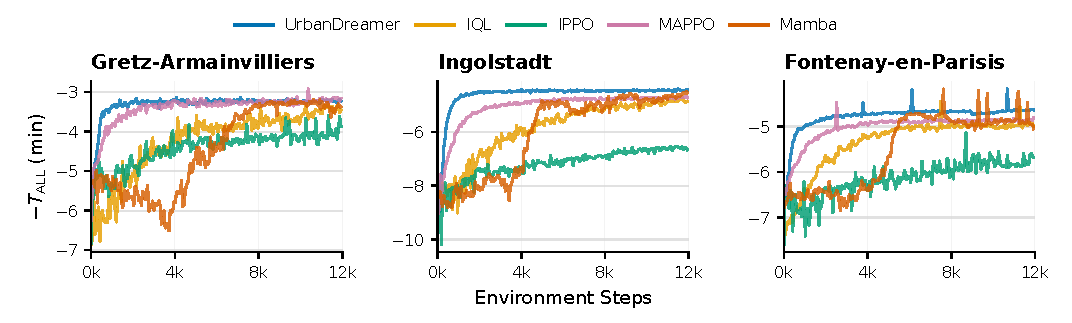
\includegraphics[width=0.8\textwidth]{figure/sample_efficiency.pdf}
  \caption{Training curves over real SUMO environment steps on the three urban networks. UrbanDreamer reaches its best moving-average $T_{\mathrm{all}}$ with 69.8\%--77.3\% fewer steps than the most sample-efficient baseline on each network.}
  \label{fig:sample-efficiency-training-proxy}
\end{figure*}



\subsubsection{Computational Efficiency}

\begin{table}[t]
  \centering
  \caption{Computational efficiency on the three urban networks. All runs use a single NVIDIA RTX 3090 GPU. Lower is better; best in bold.}
  \renewcommand{\arraystretch}{1.0}
  \setlength{\tabcolsep}{12pt}
  \begin{tabular}{lccc}
    \toprule
    \multirow{2}{*}{Method} & \multicolumn{3}{c}{Total Training Time (hours) $\downarrow$} \\
    & Gretz & Ingolstadt & Fontenay \\
    \midrule
    IQL & 28.8 & 15.3 & 78.2 \\
    IPPO & 33.0 & 10.4 & 96.1 \\
    MAPPO & 35.1 & 13.9 & 85.6 \\
    MAMBA & 37.0 & 10.2 & 78.9 \\
    \textbf{UrbanDreamer} & \textbf{17.4} & \textbf{5.6} & \textbf{33.3} \\
    \bottomrule
  \end{tabular}
  \label{tab:computation-efficiency}
\end{table}

Table~\ref{tab:computation-efficiency} reports the training time to convergence of each learning method (per-stage breakdown in Appendix~\ref{app:architecture}). UrbanDreamer completes training in 19.0, 5.4, and 36.6 hours on the three networks, reducing training time by 36.0\%, 48.1\%, and 49.2\% relative to the fastest baseline on each network.


\subsubsection{Scalability with Traffic-System Size}

\begin{figure}[t]
  \centering
  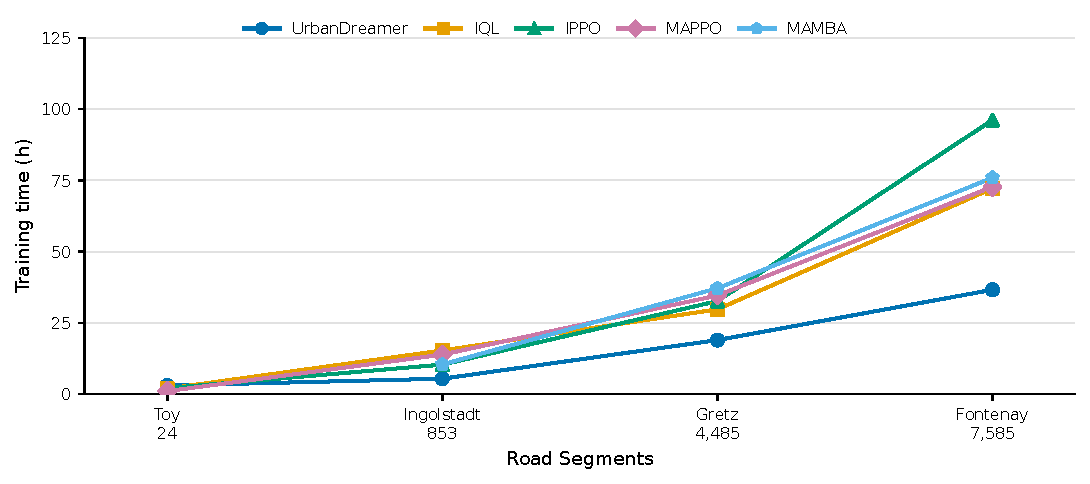
\includegraphics[width=1.0\linewidth]{figure/scalability_training_time}
  \caption{Total training time across networks of increasing size. The horizontal axis contains four discrete benchmarks ordered by road-segment count: Toy (24), Ingolstadt (853), Gretz-Armainvilliers (4,485), and Fontenay-en-Parisis (7,585). Toy is a small synthetic network used only as a pilot point in this profile. Connecting segments are visual guides rather than interpolation over a continuous scale.}
  \label{fig:scalability_training_time}
\end{figure}

Figure~\ref{fig:scalability_training_time} compares training time across networks of increasing size. Training time grows for all methods, but UrbanDreamer remains consistently faster, and its advantage widens with network size: from 5.4 hours on Ingolstadt to 36.6 hours on Fontenay-en-Parisis (7,585 segments), whereas the baselines require 72.1--96.2 hours on the largest network.

\subsection{Final Routing Quality}

\begin{table*}[t]
  \centering
  \caption{Final routing quality on the three urban networks: mean travel times in minutes for all vehicles, CAVs, and HDVs, and the 95th-percentile travel time \(T_{\mathrm{P95}}\). Lower values indicate better performance; the best value in each column is in bold.}
  \renewcommand{\arraystretch}{1.0}
  \resizebox{1.0\linewidth}{!}{
    \begin{tabular}{lcccccccccccc}
      \toprule
      \multirow{2}{*}{Method} & \multicolumn{4}{c}{Gretz-Armainvilliers} & \multicolumn{4}{c}{Ingolstadt} & \multicolumn{4}{c}{Fontenay-en-Parisis} \\
      \cmidrule(lr){2-5} \cmidrule(lr){6-9} \cmidrule(lr){10-13}
      & $T_{\mathrm{all}}\!\downarrow$ & $T_{\mathrm{CAV}}\!\downarrow$ & $T_{\mathrm{HDV}}\!\downarrow$ & $T_{\mathrm{P95}}\!\downarrow$ & $T_{\mathrm{all}}\!\downarrow$ & $T_{\mathrm{CAV}}\!\downarrow$ & $T_{\mathrm{HDV}}\!\downarrow$ & $T_{\mathrm{P95}}\!\downarrow$ & $T_{\mathrm{all}}\!\downarrow$ & $T_{\mathrm{CAV}}\!\downarrow$ & $T_{\mathrm{HDV}}\!\downarrow$ & $T_{\mathrm{P95}}\!\downarrow$\\
      \midrule
      Free-flow greedy & 3.262 & 3.537 & 3.079 & 6.667 & 4.542 & 4.590 & 4.509 & 7.333 & 4.682 & 4.676 & 4.687 & 22.651\\
      Live-current greedy & 3.331 & 3.710 & 3.079 & 6.950 & \textbf{4.410} & 4.375 & \textbf{4.433} & \textbf{6.616} & 4.691 & 4.693 & 4.690 & 22.636\\
      IQL & 3.321 & 3.687 & 3.078 & 6.867 & 4.595 & 4.785 & 4.468 & 7.416 & 4.968 & 5.552 & 4.577 & \textbf{20.947}\\
      IPPO & 3.933 & 5.169 & 3.111 & 10.569 & 5.679 & 7.532 & 4.443 & 14.693 & 5.438 & 6.611 & 4.657 & 25.171\\
      MAPPO & 3.246 & 3.538 & \textbf{3.050} & 6.617 & 4.664 & 4.867 & 4.528 & 7.533 & 4.838 & 5.245 & 4.566 & 22.928\\
      MAMBA & 3.353 & 3.725 & 3.106 & 6.867 & 4.555 & 4.519 & 4.578 & 7.016 & 5.068 & 5.821 & 4.566 & 23.233\\
      \textbf{UrbanDreamer} & \textbf{3.167} & \textbf{3.297} & 3.081 & \textbf{6.583} & 4.421 & \textbf{4.370} & 4.454 & 6.883 & \textbf{4.600} & \textbf{4.665} & \textbf{4.556} & 22.285\\
      \bottomrule
    \end{tabular}
  }
  \label{tab:overall-performance}
\end{table*}


Table~\ref{tab:overall-performance} reports final routing quality on the three networks. UrbanDreamer attains the lowest global mean travel time on Gretz-Armainvilliers and Fontenay-en-Parisis; on Ingolstadt it is second to live-current greedy by 0.01 minutes and lowest among the learning-based methods. The gains come primarily from lower CAV travel times, and UrbanDreamer also incurs the lowest added cost \(C_{\mathrm{ALL}}\) on all three networks.


\subsection{Ablation}

We conduct three groups of ablations: component ablation on final routing quality, efficiency ablation isolating world-model imagination, and transition ablation comparing predictive quality across transition models.

\subsubsection{Component Ablation}

We compare UrbanDreamer with four variants: Actor-Critic removes world-model imagination, w/o HDV Response removes HDV influence prediction, Vehicle Critic Only retains only the per-vehicle critic, and MSE Transition replaces flow matching with deterministic next-state regression.

\begin{table*}[t]
  \centering
  \caption{Component ablation: final mean travel times in minutes when individual components are removed or replaced. Lower values indicate better performance.}
  \renewcommand{\arraystretch}{1.0}
  \resizebox{1.0\linewidth}{!}{
    \begin{tabular}{lccccccccc}
      \toprule
      \multirow{2}{*}{Method} & \multicolumn{4}{c}{Gretz-Armainvilliers} & \multicolumn{4}{c}{Ingolstadt} & \multicolumn{4}{c}{Fontenay-en-Parisis} \\
      \cmidrule(lr){2-5} \cmidrule(lr){6-9} \cmidrule(lr){10-13}
      & $T_{\mathrm{ALL}}\!\downarrow$ & $T_{\mathrm{CAV}}\!\downarrow$ & $C_{\mathrm{ALL}}\!\downarrow$ & $T_{\mathrm{P95}}\!\downarrow$ & $T_{\mathrm{ALL}}\!\downarrow$ & $T_{\mathrm{CAV}}\!\downarrow$ & $C_{\mathrm{ALL}}\!\downarrow$ & $T_{\mathrm{P95}}\!\downarrow$ & $T_{\mathrm{ALL}}\!\downarrow$ & $T_{\mathrm{CAV}}\!\downarrow$ & $C_{\mathrm{ALL}}\!\downarrow$ & $T_{\mathrm{P95}}\!\downarrow$\\
      \midrule
      Actor-Critic & 3.219 & 3.514 & 0.942 & 6.852 & 4.572 & 4.764 & 4.443 & 4.771 & 5.114 & 4.543 \\
      w/o HDV Response & 3.284 & 3.624 & 0.364 & 6.450 & 4.507 & 4.522 & 4.497 & 4.704 & 4.919 & 4.561 \\
      Vehicle Critic Only & 3.272 & 3.580 & 0.342 & 6.467 & 4.451 & 4.378 & 4.497 & 4.673 & 4.864 & 4.546 \\
      MSE Transition & 3.240 & 3.479 & 3.081 & 0.375 & 6.550 & 4.518 & 4.514 & 4.682 & 4.862 & 4.563 \\
      \textbf{UrbanDreamer} & \textbf{3.167} & \textbf{3.297} & \textbf{0.230} & \textbf{6.583} & 4.421 & \textbf{4.370} & \textbf{0.146} & 6.883 & \textbf{4.600} & \textbf{4.665} & \textbf{-0.295} & 22.285\\
      \bottomrule
    \end{tabular}
  }
  \label{tab:ablation performance}
\end{table*}


Table~\ref{tab:ablation performance} shows that removing any component degrades routing performance on all three networks. Removing world-model imagination causes the largest degradation on Ingolstadt and Fontenay-en-Parisis, while removing the HDV response module is most harmful on Gretz-Armainvilliers. Replacing flow matching with MSE regression also degrades both routing performance and prediction quality (Table~\ref{tab:wm-prediction-ablation}).

\subsubsection{Efficiency Ablation}

\begin{figure*}[t]
  \centering
  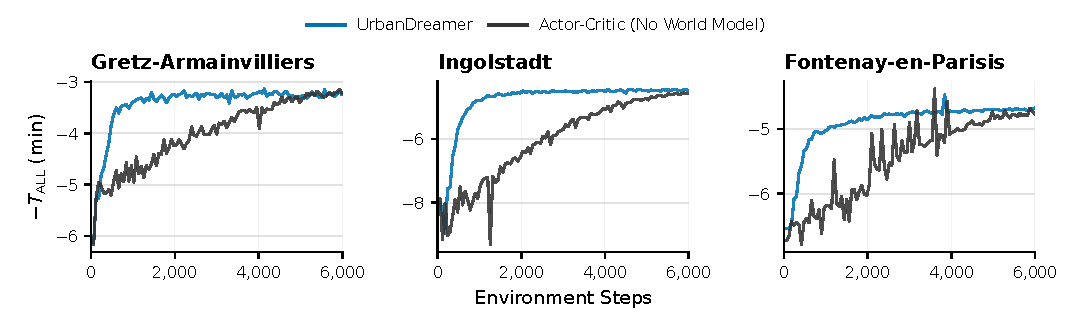
\includegraphics[width=0.8\linewidth]{figure/efficiency_ablation}
  \caption{Sample-efficiency ablation on three urban road networks. The training curves compare UrbanDreamer with Actor-Critic (No World Model) over real SUMO environment steps. Higher \(-T_{\mathrm{all}}\) indicates better routing performance.}
  \label{fig:efficiency_ablation}
\end{figure*}

Figure~\ref{fig:efficiency_ablation} compares UrbanDreamer with Actor-Critic (No World Model) over real environment steps. UrbanDreamer improves substantially faster and stabilizes with fewer steps on all three networks, demonstrating that world-model imagination drives the sample-efficiency gain.

\subsubsection{Transition Ablation}

We compare the flow-matching transition with its MSE-based counterpart on held-out 8-step rollouts, measuring the MAE of normalized speed and capacity-normalized vehicle count.

\begin{table}[t]
  \centering
  \caption{8-step frozen-trace prediction error (lower is better).}
  \renewcommand{\arraystretch}{1.0}
  \resizebox{\columnwidth}{!}{%
    \begin{tabular}{lcccc}
      \toprule
      \multirow{2}{*}{Network} & \multicolumn{2}{c}{Speed MAE $\downarrow$} & \multicolumn{2}{c}{Vehicle Count MAE $\downarrow$} \\
      \cmidrule(lr){2-3} \cmidrule(lr){4-5}
      & Flow Matching & MSE Loss & Flow Matching & MSE Loss \\
      \midrule
      Ingolstadt & \textbf{0.408} & 0.433 & \textbf{0.060} & 0.066 \\
      Gretz-Armainvilliers & \textbf{0.274} & 0.473 & \textbf{0.104} & 0.125 \\
      Fontenay-en-Parisis & \textbf{0.209} & 0.233 & \textbf{0.107} & 0.112 \\
      \bottomrule
    \end{tabular}%
  }
  \label{tab:wm-prediction-ablation}
\end{table}

Table~\ref{tab:wm-prediction-ablation} shows that flow matching achieves lower speed and vehicle-count MAE on all three networks, demonstrating more accurate multi-step transition prediction.
